
\subsection{Bootstrap and Lifecycle}

The different components of the system runs independently from each other. However, still, connection needs to be established to form the whole system. The said connections are not created eagerly, though, as to avoid the looping issues with (possible) cyclic dependency and to reduce the bootstrap time.

For the front-ends, as they are only created when needed, they do not to fit in the bootstrap stage. They will be able to work fine as long as the system is online at the time of use. 

The structure of the system suggests the explicit dependencies of the system:

\begin{itemize}
	\item The API is dependent on the Persistent Storage as the API does not hold any data at the time of bootstrap.
	\item The API and Lambda depend on the Key Value Store.
\end{itemize}

and the implicit ones:

\begin{itemize}
	\item S3 should be present whenever API and Lambda is available as it serves as a mean to invoke the Lambda instances for the API.
	\item We have used the Redis (Key Value Store engine) Channel for Lambda state monitoring.
\end{itemize}

Topologically a reasonable bootstrap order, then, would be\footnote{That is, we sort the items based on a order that takes the dependencies into consideration. For more information regarding topological sort please see https://en.wikipedia.org/wiki/Topological\_sorting.}.

\begin{enumerate}
	\item[1] Persistent Storage Unit
	\item[1] Key Value Store
	\item[2] The API
	\item[3] Lambda\footnote{Lambda is quite special in terms of lifecycle. See below for detailed information.}
\end{enumerate}

where the order of items with the same number are inter-exchangeable.

Different components behave in different manners, in terms of its lifecycle:

\begin{itemize}
	\item The API resides inside Docker running on EC2. The actual deployment, scaling and provisioning are done through AWS Elastic Beanstalk~\cite{beanstalk}. We have also assumed that unless under special cases such as necessary offline maintenance or system upgrading, the service will not be offline. AWS Beanstalk will automatically re-boot the API if, under exceptional circumstances, the API goes down.
	\item The nature of persistence of the API naturally requires the persistence of the Persistent Storage Unit and Key Value Storage. Fortunately, due to the use of AWS RDS, S3 and ElastiCache there is no need for manual management of the components lifecycle.
	\item Lambda is a special type of unit. Lambda instances are only fired up whenever there is a cattle registration or match request coming in, and will be instantly destroyed/disregarded when the computation is done to save the resources. Lambda instances then have a very short lifecycle, and are fairly lightweight to bootstrap\footnote{In fact the bootstrap of each Lambda instance only requires the the connection to the Key Value Store. This process takes little to no time as they both are close both geographically and in the network.}.
\end{itemize}

Unfortunately, under certain cases, the services might have to be shut down. The order of shut down is rather different compare to that of bootstrap:

\begin{enumerate}
	\item The API needs to be notified first, as to stop accepting new requests.
	\item If there are running Lambda instances, wait for them to run to finish. This is acceptable as Lambda instances are programmed as lightweight computational units and generally a very small (~15 seconds) running time limit is imposed on all Lambda instances.
	\item The Persistent Storage Unit.
	\item The Key Value Store. However, extra care must be taken in the shutdown process of the Key Value Store to keep the data. Fortunately it is being backed up daily and at time of shutdown automatically.
\end{enumerate}

\subsection{Use of ElastiCache}

Unlike the name suggests, ElastiCache is not employed as a cache engine from a programming point of view, because we have assumed that the saved key-value pairs will always be available unless otherwise indicated. In our design the system uses Redis, the Key-Value storage to store the descriptors to reduce the running time of the matching process - a suggestion of, from a philosophical point of view, a caching process.

From the previous subsection it is pointed out that the data in the key-value store is being kept. This is not the ideal use case of any cache engine; however, in the future iterations, it has been agreed on that the system will handle the cache miss should it ever happen as a way to make the system more robust.

\subsection{Use of S3}

Our system has been using S3 extensively. There are two main uses for S3:

\begin{itemize}
	\item Image storage: images of cattle are saved onto S3. The index include the cattle ID and the image ID. User ID does not constitute part of the key as a cattle does not belong to one and only one owner.
	\item Action trigger. Object creation/update and deletion on S3 turns out to be able to send a notification message to the other Amazon cloud services.
\end{itemize}

One reason that S3 has been used as a simple action trigger service is that as it turns out, S3 has a much more robust connection with the rest of the Amazon Cloud services. The original implementation of the Job Assignment Lambda invokes the Matching Lambda with the official AWS SDK \texttt{boto3}, however that seemed to be unusable. The Job Assignment Lambda has a running time limit of 10 seconds, however the invocation process using \texttt{boto3} alone frequently bring the whole process to timeout\footnote{Our speculation is that it might be the \texttt{Payload} data that we are sending is over 500KB - a scenario that \texttt{boto3} is not optimised for.}. After some testing and digging around, we found out that if we save the parameter (the descriptor for the image to be matched against) onto S3 as an object, and if that triggers the invocation of the Matching Lambda, the problem would be resolved and it is lightning fast and there never had been any connection issues. We have decided to keep using S3 since after some debate for the non-ideal use of the service.

\subsection{Algorithm Performance}
\label{sec:algorithm}

It has been briefly discussed about the algorithm performance and the discussion will resume at this section. Note that the following tests are concluded on a machine with the 

\begin{itemize}
	\item Processor: Intel Core i7-6820HQ, 2.7 GHz, 4 cores, 8 processes
	\item Memory: 16 GB 2133 MHz LPDDR3
	\item Operating System: macOS 10.12.2 (build 16C67)
\end{itemize}

and GPU acceleration turned off.

A simple test (with a sample size of 144 pairwise image matches) yields the following result, note that the edge and descriptor generation are for two images (unit: ms):

\begin{center}
\begin{tabular}{c|c c c}
        & Edge Generation & Descriptor Generation & Matching \\
\hline
Mean    & $135.20$       & $482.91$              & $47.15$  \\
Medium  & $136.68$       & $450.11$              & $42.77$  \\
SD      & $11.87$        & $91.72$               & $28.79$
\end{tabular}
\end{center}

Note that edge and descriptor generation are only done once for each request. The total time then is bound by the formula $N * t_m + t_d$ where $N$ is a fixed number, ignoring the time for IO actions. The running time is not upper bounded by the data size even though the matching process is essentially pairwise as an important assumption we have made is that we always have as many Lambda instances at our disposal as we want by our design.

An box-plot visualisation of the data is shown in the combined plot ~\ref{fig:algo_visual_all}.

\begin{figure}[H]
	\centering
	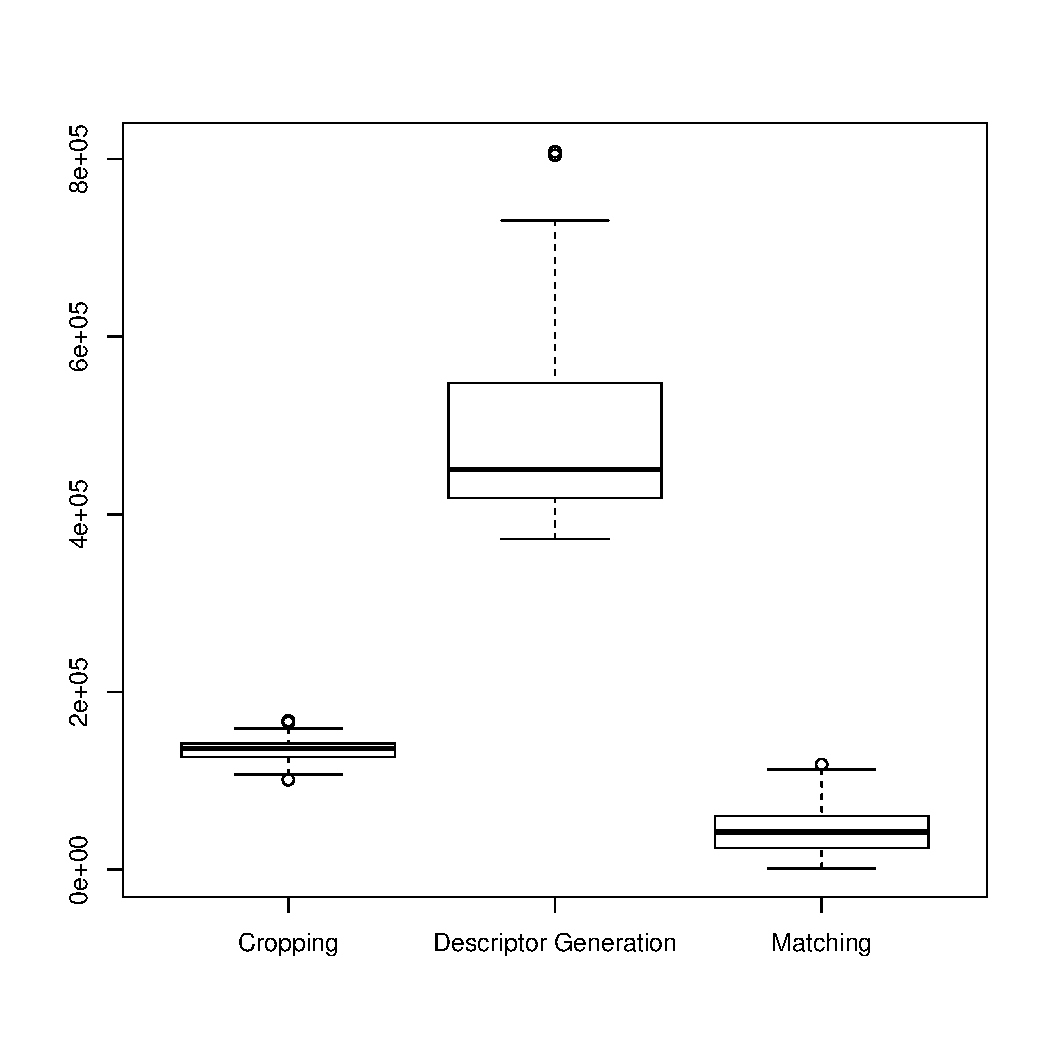
\includegraphics[width=0.8\textwidth]{sketch/all.pdf}
	\caption{The combined algorithm runtime plot}
	\label{fig:algo_visual_all}
\end{figure}

The visualisation clearly suggests that the runtime of the algorithm is rather stable all but for the descriptor generation process. This proves that the runtime will be acceptable in our case for a pairwise matching.

\subsection{Performance of Serverless Architecture}

There is a serious issue with performance loss on the serverless AWS  serious issue here is performance, especially in the thinning process\footnote{Zhang-Suen thinning algorithm.} as the computational task is quite substantial. In this special case, it is required to inline C++ code as opposed to having pure Python code for the thinning iteration\footnote{The inline version runs within 600ms with IO whereas the pure Python version just times out after 10 seconds.}. The recommended approach is to use \texttt{weave} from \texttt{scipy} to inline the small piece of code. However this has proven to be not so easy: AWS Lambda has a (code) package size limit of 250MB, and \texttt{scipy} itself is over 200MB - this implies that there is no way that we can use \texttt{scipy}.

Since we only need to use \texttt{weave}, we installed it as an independent library. However, we found that since \texttt{weave} uses \texttt{scipy} internally, this was not a solution at all and we were back to square one.

We were left with no choice but to manually compile the C++ code into an object file for Python to use. Fortunately this is not too difficult: we needed to run the code with \texttt{weave.inline} on a compatible machine and grab the \texttt{weave}-generated C++ file from the cache. For every platform we require, we compile it into an object file and store it in the \texttt{lib} directory. This works because \texttt{weave} generates the boilerplate for seamless Python integration. After this step we would be able to replace the code with a call to the generated function in the generated module and remove the requirements for \texttt{weave} and \texttt{scipy}.

\subsection{Maintaining Security}

Part of the brief for this project was to maintain the security of the intellectual property created at all times. When deploying the application, this sometimes resulted in a debugging process which was very obfuscated owing to the closed-down nature of what we deployed. For example, we chose to not have SSH access into our API gateway instances in order to reduce the attackable surface area.

Furthermore, all data for the application is contained within a private subnet within a virtual private cloud such that it has no direct connection to the internet, and therefore is not subject to attack. This made some parts of deployment difficult, since our network configuration had to be created such that the compute elements of the system were able to be accessed from the internet, whilst connecting to and using data from the internet-inaccessible data layer.

By using AWS IAMs, we were able to further isolate the abilities of individual actors in the system, reducing the attack surface to it's minimum, and providing a means to determine the exact source of an attack should one occur.

\subsection{Infrastructure Financial Constraints}

One of the key problem sources during our project was infrastructure. The infrastructure was the only part of the project which would have a cost directly attached to it. We were given available hardware through the university's hardware program exposing a choice of machines running through Apache CloudStack. We started our project with these machines, finding deployment to be very time consuming and unreliable. Furthermore, owing to the modern technologies we deployed, some software, such as GitLab CI, seemed unoptimised and ran incredibly slowly, further delaying deployment and iterations.

Therefore, as the project progressed, we researched using professional cloud service providers which offered completely custom software, some of which would largely handle deployment in an automated fashion. We researched using both Microsoft Azure and Amazon Web Services (AWS) \footnote{Credits were available for both platforms through a university affiliation program.}, eventually choosing AWS for it's superior software package and unrivalled functionality in AWS lambda. 

Using AWS lambda, a pure functional environment designed to be deployed as a software package and be triggered and executed in parallel across hundreds of machines gave us performance that we couldn't hope to emulate without many more hours of development, deployment, and financial burden. With low cost pricing and a generous free allowance \footnote{AWS provides 3,200,000 GB/seconds for free per month as part of it's free tier at the time of writing}, we were able to develop an instantly scalable, efficient system to provide the backbone of our image processing and identification.

The experience of using multiple providers in this scenario brought a clear conclusion. Whilst for all intents and purposes each provider is offering some identical unit of compute at slightly different price points, the implementation and use of that unit of compute differs astronomically through the software layer atop the hardware. It would be unfathomable to conceive a competitor to AWS lambda running on commodity hardware in the time period available to this project, and consequently, the group found that in order to make the project a success we were somewhat required to use paid services.

Before transitioning to using AWS, backed by GitHub and CircleCI for version control and continuous integration respectively, the proportion of our time we spent on deployment and systems issues was vastly higher than we would have liked. After moving to AWS, this time became nominal as we were able to rely on a dependable platform for service delivery.

In conclusion, should we have remained with the provided commodity hardware using a basic software layer, we wouldn't have had a financial burden but we wouldn't have achieved the success that we have with the project either. 

